Перед Вами – необычное издание. Это лекции \href{https://dlnp.jinr.ru/news/618}{Егорова Вячеслава Георгиевича} по общей физике, которые он читал студентам \href{https://www.uni-dubna.ru/}{университета «Дубна»}.

Доктор физико-математических наук, начальник сектора отдела НЭОЯСиРХ ОИЯИ, профессор кафедры физики университета «Дубна» Егоров Вячеслав Георгиевич был выдающимся физиком, представителем того редкого и почти исчезнувшего вида ученых, которые способны самостоятельно выполнить физический эксперимент от начала и до конца. От идеи, поставновки задачи через создание установки к проведению измерений и завершая анализом данных, получением результатов и написанием статьи. Нужно отметить, что в современной науки чаще всего существует явная специализация, есть эксперты по электронике, написанию ПО, симуляциям, обработке данных. Безусловно, этому способствует неизбежная глобализация в науке – все ведущие направления исследований требуют создания огромных установок – научных фабрик, в которых заняты сотни и тысячи ученых. Тот же Слава говорил «все простые законы, которые лежали, уже давно расхватали. Это раньше можно было взять магнит и проволоку, открыть закон, назвав его своим именем. А теперь нужно сильно напрягаться и копать глубоко». Но, все равно, универсализм и умение мастеров на все руки все еще вызывает истинное восхищение и уважение.

И второй важный момент, имеющий прямое отношение к данной книге – Слава был Учителем с большой буквы, он всегда умел объяснить сложные вещи простыми словами, находить удачные и точные образы, проявляя при этом удивительную находчивость и смекалку. Способности Славы как нельзя лучше передает жизненная история, случившаяся с нами в большом французском супермаркете, где мы искали лавровый лист и никак не могли найти. Тогда Слава подозвал девушку-работника магазина и попытался поговорить с ней на английском. Но она его не поняла. Тогда Слава, недолго думая, взял в руки воображаемый лавровый венок, торжественно надел его себе на голову и стал в позу Наполеона. Девушка засмеялась и тут же отвела нас к стойке со специями.

Я сам не знал об этих лекциях, но услышал о них впервые от своего коллеги \href{https://www.utef.cvut.cz/staff/00078/ivan-stekl}{Ивана Штекла}, который после ухода Славы сказал «у Славы были отличные лекции по физике, которые жалко было бы потерять». И вот, разбирая электронные документы с его компьютера я наткнулся на папку lectures. Каждая лекция была в отдельной папке, в формате LaTeX, огромное количество оригинальных рисунков, формул – и это все было сделано вручную, до эпохи chatGPT и MidJourney… Тут понимаешь,что на это были потрачены десятки, если не сотни часов времени – Слава, как всегда, если брался за что-то, то делал это на совесть, а также с присущим ему страстью и энтузиазмом.

Лекции сохранены в практически оригинальном стиле автора, с небольшими техническими изменениями,  связаными с компоновкой в единую книгу. Несколько первых глав были отформатированы в универсальном стиле книги, но потом я бросил эту затею, потому что уникальный авторский стиль просто невозможно подогнать под стандарт. Во-первых, это потребует большого объема работы, во-вторых, это уже будет другой документ. Поэтому пусть все останется так, как было задумано и реализовано автором.

Это не обычный канонический фундаментальный курс общей физики, пытающийся охватить все темы подробно. Наоборот, это выжимка, дайджест, избранные главы, экстракт наиболее важных, по мнению автора, физических понятий, которые необходимо знать студенту. Это своеобразная \sout{книжка-комикс}, \sout{книжка-раскраска}, книжка-презентация с яркими картинками и интересными примерами. Уверен, что каждый найдет в ней что-то интересное. Студент может использовать для обучения. Специалист – может увидеть уже известные ему вещи с иной стороны, под иным углом зрения. Как та девушка, увидевшая Наполеона в лавровом венке...

Удачного прочтения!

{\bf Шитов Ю.А.}

\centering
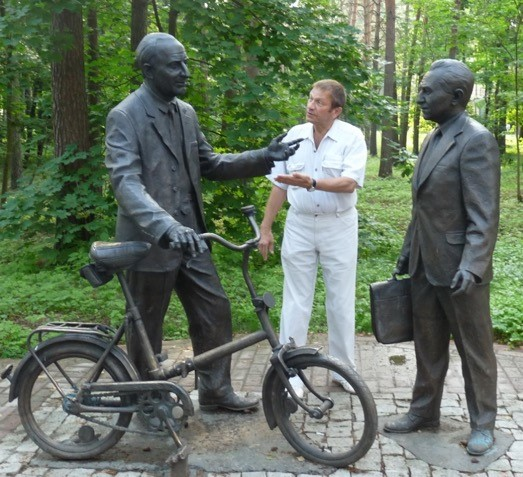
\includegraphics[width=0.9\textwidth]{photos/egorov_pontecorvo_djelepov.jpg}

Вячеслав Георгиевич обсуждае курс лекций по общей физике с Бруно Понтекорво и Венедиктом Петровичем Джелеповым.
